\section{Adversarial Control Experiments}
\label{sec:phys_exps}

\noindent\textit{ViMo-Flow motion-generation experiments along with spml (34-joints) to deepmimic (24-joints) retargeting convertion scope is convered here: Appendix~\ref{sec:vimo_exps}.}\par

\subsection{Implementation details}
Controller training ran for 5,000 epochs in MuJoCo at 30 FPS. Two rollout settings were evaluated: horizon $H_{\text{steps}}=8$ with 32 parallel environments, and horizon $H_{\text{steps}}=16$ with 16 parallel environments. PPO used 5 update epochs per rollout, clip ratio $\epsilon=0.2$, discount $\gamma=0.95$, and GAE parameter $\lambda=0.95$~\cite{ppo2017}. Learning rates were fixed at $5\times 10^{-6}$ for the actor, $10^{-4}$ for the critic, and $10^{-5}$ for the discriminator. Gradient penalty used $\lambda_{\text{gp}}=10$~\cite{wgangp2017}, and symmetry experiments used $\lambda_{\text{sym}}=0.005$~\cite{symlocom2018}. The adversarial reward followed the ICCGAN-style discriminator setup used in the control framework~\cite{iccgan2021, composite2023}.

\paragraph{Reference motions and difficulty tiers.}
The evaluation focused on three single-clip locomotion motions with increasing control difficulty:
\begin{itemize}
    \item \textbf{limp\_walk}: slow, ground-contact dominated, no aerial phase;
    \item \textbf{joyful\_walk}: moderate pace with mild vertical impulse;
    \item \textbf{jaunty\_walk}: high-energy, fast, and visibly asymmetric.
\end{itemize}
The corresponding step counts per motion cycle were 57 for \textit{limp\_walk}, 35 for \textit{joyful\_walk}, and 41 for \textit{jaunty\_walk}, as parsed from the environment configuration. Maximum episode length was set to two cycles for \textit{limp\_walk} and \textit{joyful\_walk}, and one cycle for \textit{jaunty\_walk}. In addition to these controlled case studies, feasibility of the full pipeline was checked on retargeted motion clips generated by the motion synthesis model and stored under the `vimo` motion set.

\subsection{Evaluation metrics}
For a motion with cycle length $S_{\text{cycle}}$, the normalized survival metric is
\[
    \text{lifetime\_cycles} = \frac{\text{lifetime}}{S_{\text{cycle}}}.
\]
Discriminator quality was tracked through mean real score, mean fake score, and their gap,
\[
    \text{disc\_gap} = \text{score}_{\text{real}} - \text{score}_{\text{fake}}.
\]
Additional diagnostics included mean reward, policy loss, value loss, and normalized symmetry loss when symmetry regularization was active. Metrics were summarized over the final training window (epochs 4500--5000), matching the procedure used in the case-study summaries.

\paragraph{Baseline performance.}
The baseline runs without phase input and without symmetry loss established the reference operating point. At $H=8$, final survival reached $0.68 \pm 0.08$ cycles for \textit{limp\_walk}, $0.43 \pm 0.05$ cycles for \textit{joyful\_walk}, and $0.29 \pm 0.04$ cycles for \textit{jaunty\_walk}. At $H=16$, the corresponding baselines were $0.56 \pm 0.09$, $0.46 \pm 0.07$, and $0.23 \pm 0.05$ cycles. This ordering is consistent with the qualitative difficulty of the three motions: the easier, contact-dominated gait survives longer, while faster and more asymmetric clips remain harder to stabilize.

\paragraph{Horizon ablation ($H=8$ versus $H=16$).}
Increasing the rollout horizon improves the temporal support available to the critic and the discriminator, but it also reduces the number of environments collected per update in the present setup. The effect was motion dependent. For \textit{limp\_walk}, the phase-input variant improved from $0.69 \pm 0.09$ cycles at $H=8$ to $0.73 \pm 0.11$ cycles at $H=16$, indicating that longer temporal context is beneficial when the motion is periodic and stable. For \textit{joyful\_walk}, the symmetry variant improved from $0.71 \pm 0.08$ cycles at $H=8$ to $0.77 \pm 0.13$ cycles at $H=16$. For \textit{jaunty\_walk}, however, the best result remained phase-based and only changed from $0.38 \pm 0.05$ to $0.33 \pm 0.06$, showing that horizon extension alone does not resolve strongly asymmetric or impulsive control demands.

\subsection{Case study I: phase-conditioned observations}

Phase input augments the observation vector with sinusoidal encodings of the normalized cycle position:
\[
    \mathbf{s}_t^{\text{phase}} = \begin{bmatrix} \mathbf{s}_t \\ \sin(2\pi\phi_t) \\ \cos(2\pi\phi_t) \end{bmatrix}, \quad \phi_t = \frac{t \mod S_{\text{cycle}}}{S_{\text{cycle}}},
\]
where $\phi_t \in [0,1]$ denotes the phase within the motion cycle. This conditioning provides explicit temporal alignment cues that reduce ambiguity in reference-following for periodic motions.

\textbf{Limp walk results.} At $H=8$, phase conditioning improved:
\begin{itemize}
    \item Mean reward: $-0.0901 \rightarrow -0.0644$ ($28.5\%$ improvement)
    \item Discriminator gap: $0.2718 \rightarrow 0.2658$
    \item Lifetime cycles: $0.68 \rightarrow 0.69$ (marginal gain)
\end{itemize}
At $H=16$, the phase variant achieved the best configuration with $0.73 \pm 0.11$ cycles and reward $-0.0505$, confirming that extended temporal context combined with phase information benefits stable locomotion.

\begin{figure}[htbp]
    \centering
    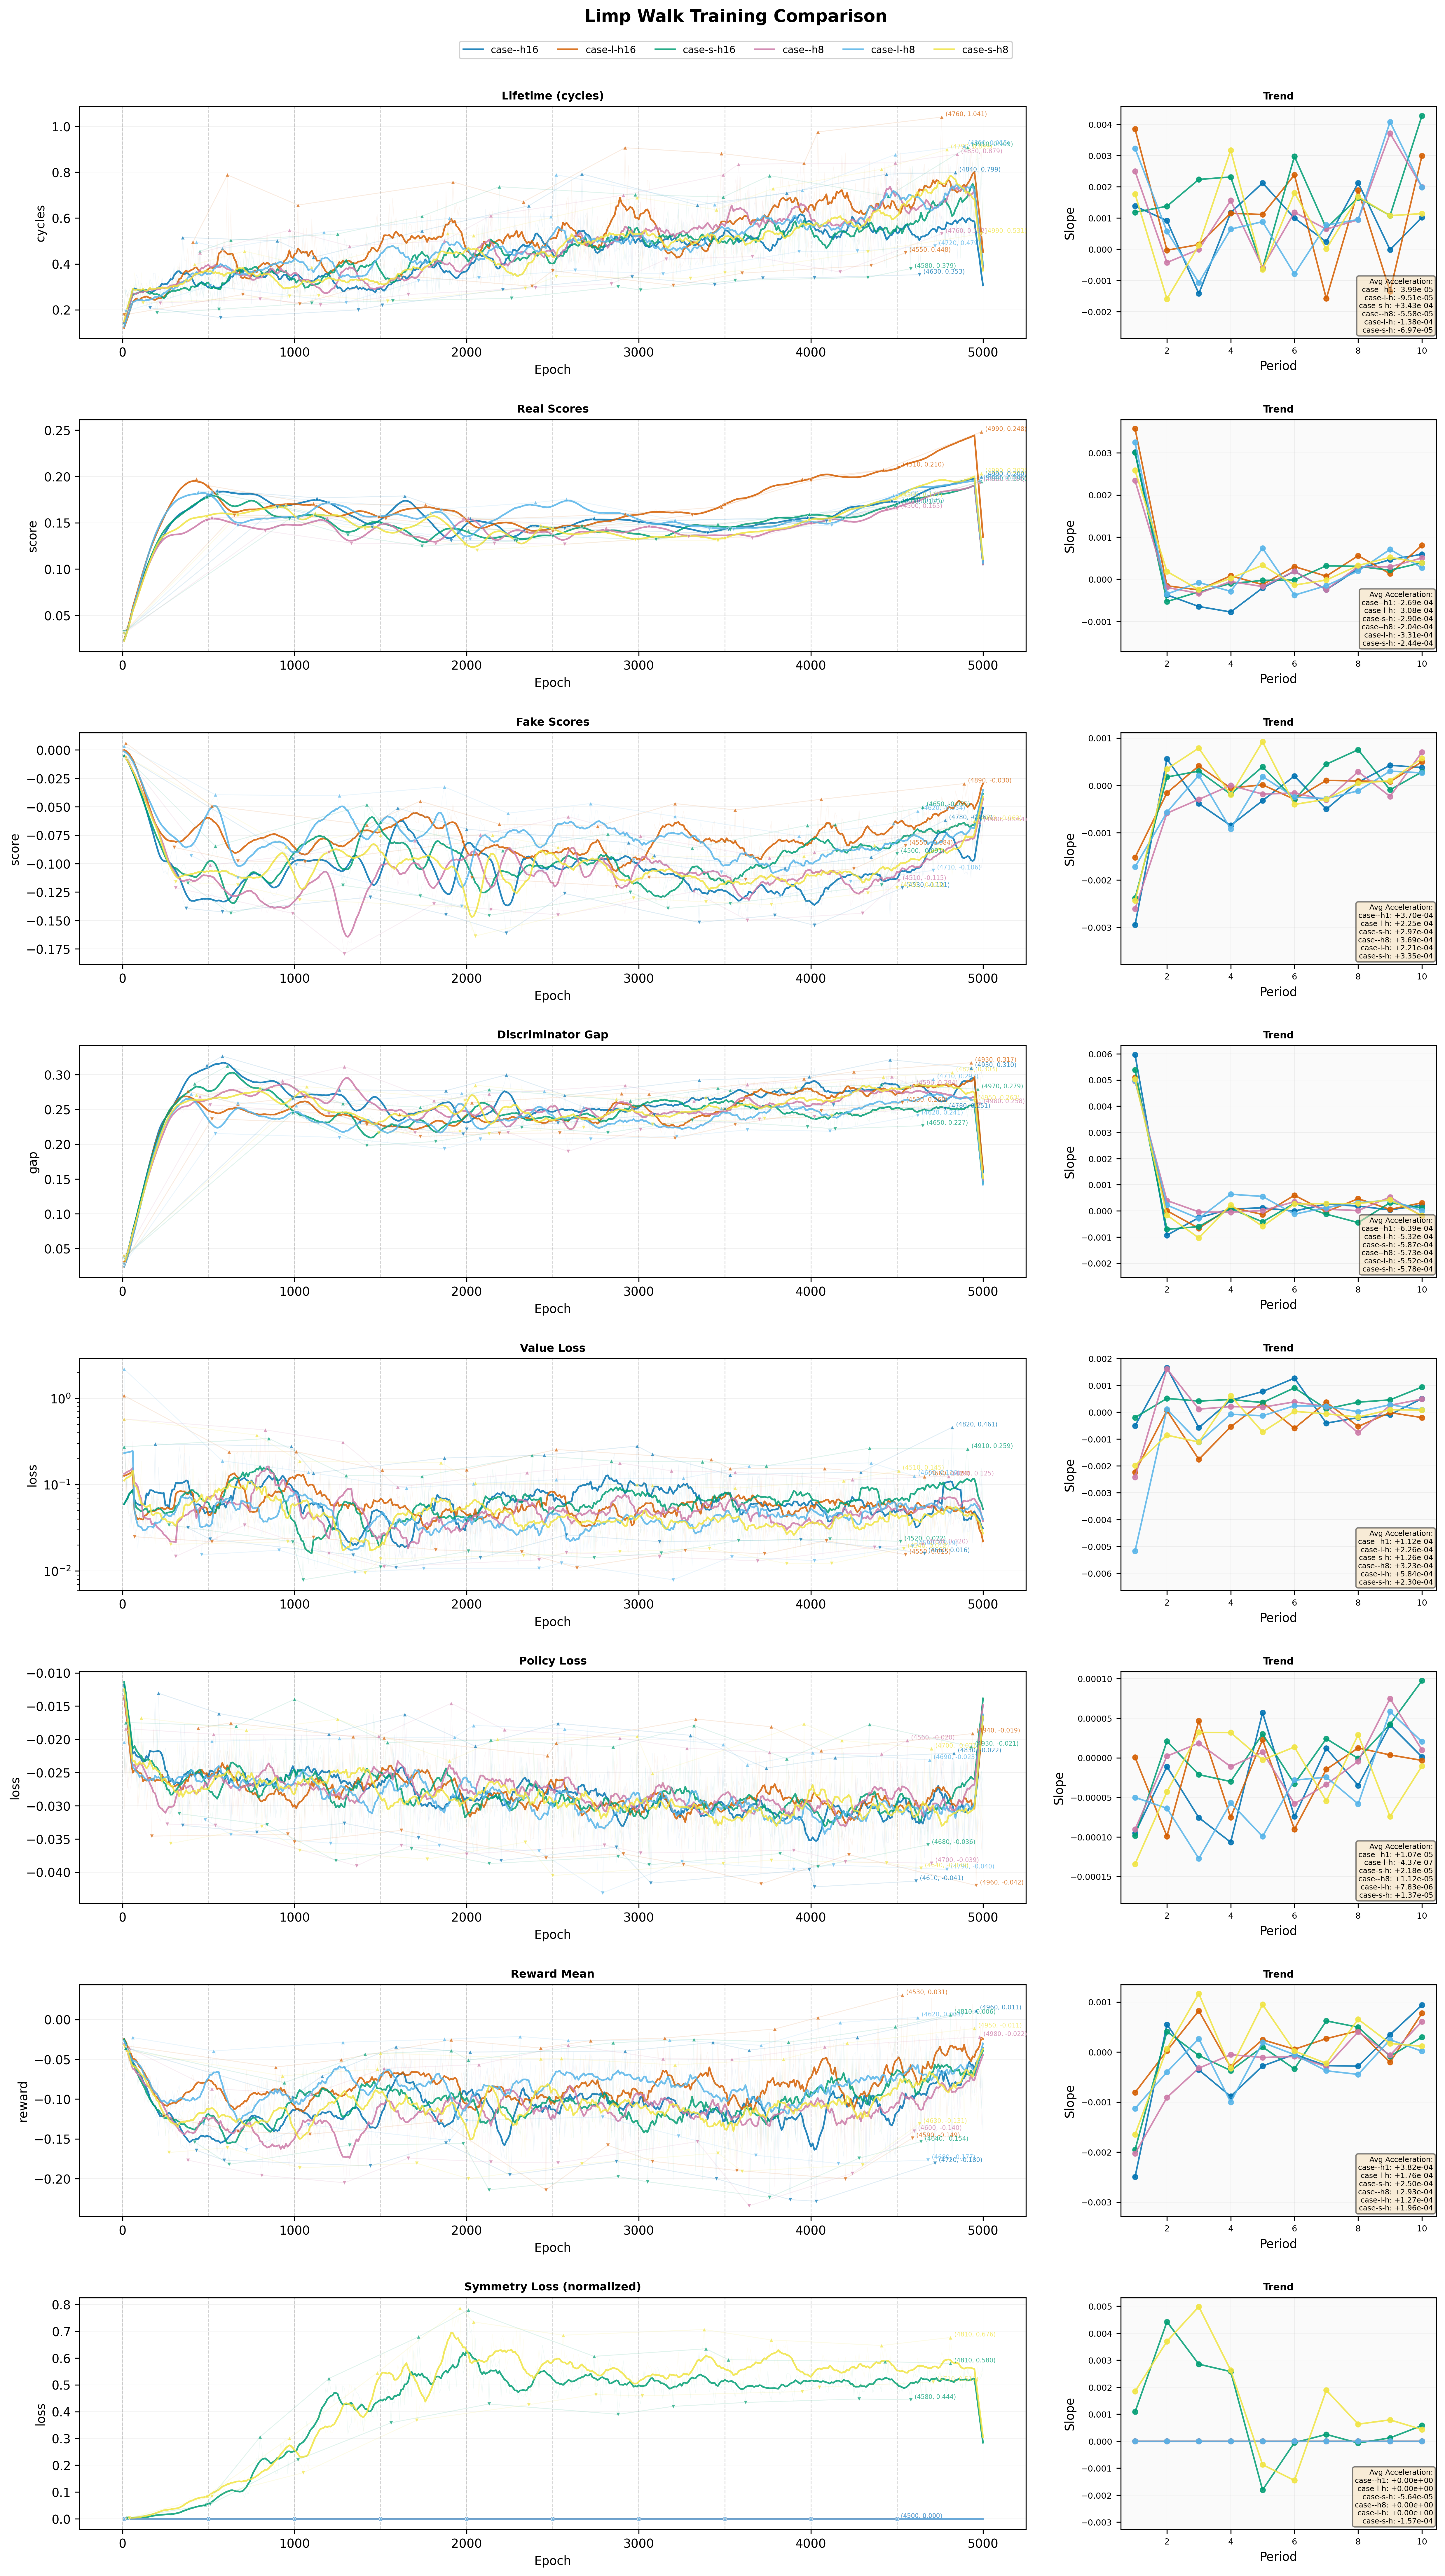
\includegraphics[height=.925\textheight, keepaspectratio]{outputs/case_studies/limp-h=8,16.png}
    \caption{Limp walk training comparison across baseline (\texttt{baseline}), phase-input (\texttt{phase}), symmetry-regularized (\texttt{sym}), and combined (\texttt{phase+sym}) variants at $H=8$ and $H=16$. Metrics include lifetime cycles, discriminator scores, gap, value loss, policy loss, reward mean, and normalized symmetry loss.}
    \label{fig:limp_case}
\end{figure}

\textbf{Jaunty walk results.} For the asymmetric high-energy motion, phase conditioning produced the strongest gains among all implemented variants:
\begin{itemize}
    \item At $H=8$: lifetime $0.29 \pm 0.04 \rightarrow 0.38 \pm 0.05$ cycles ($31\%$ improvement)
    \item Reward: $-0.0925 \rightarrow -0.0349$ ($62.3\%$ improvement)
    \item Fake discriminator score: $-0.0646 \rightarrow -0.0126$ (closer to real)
    \item At $H=16$: maintained advantage at $0.33 \pm 0.06$ vs. $0.23 \pm 0.05$ baseline
\end{itemize}

\begin{figure}[htbp]
    \centering
    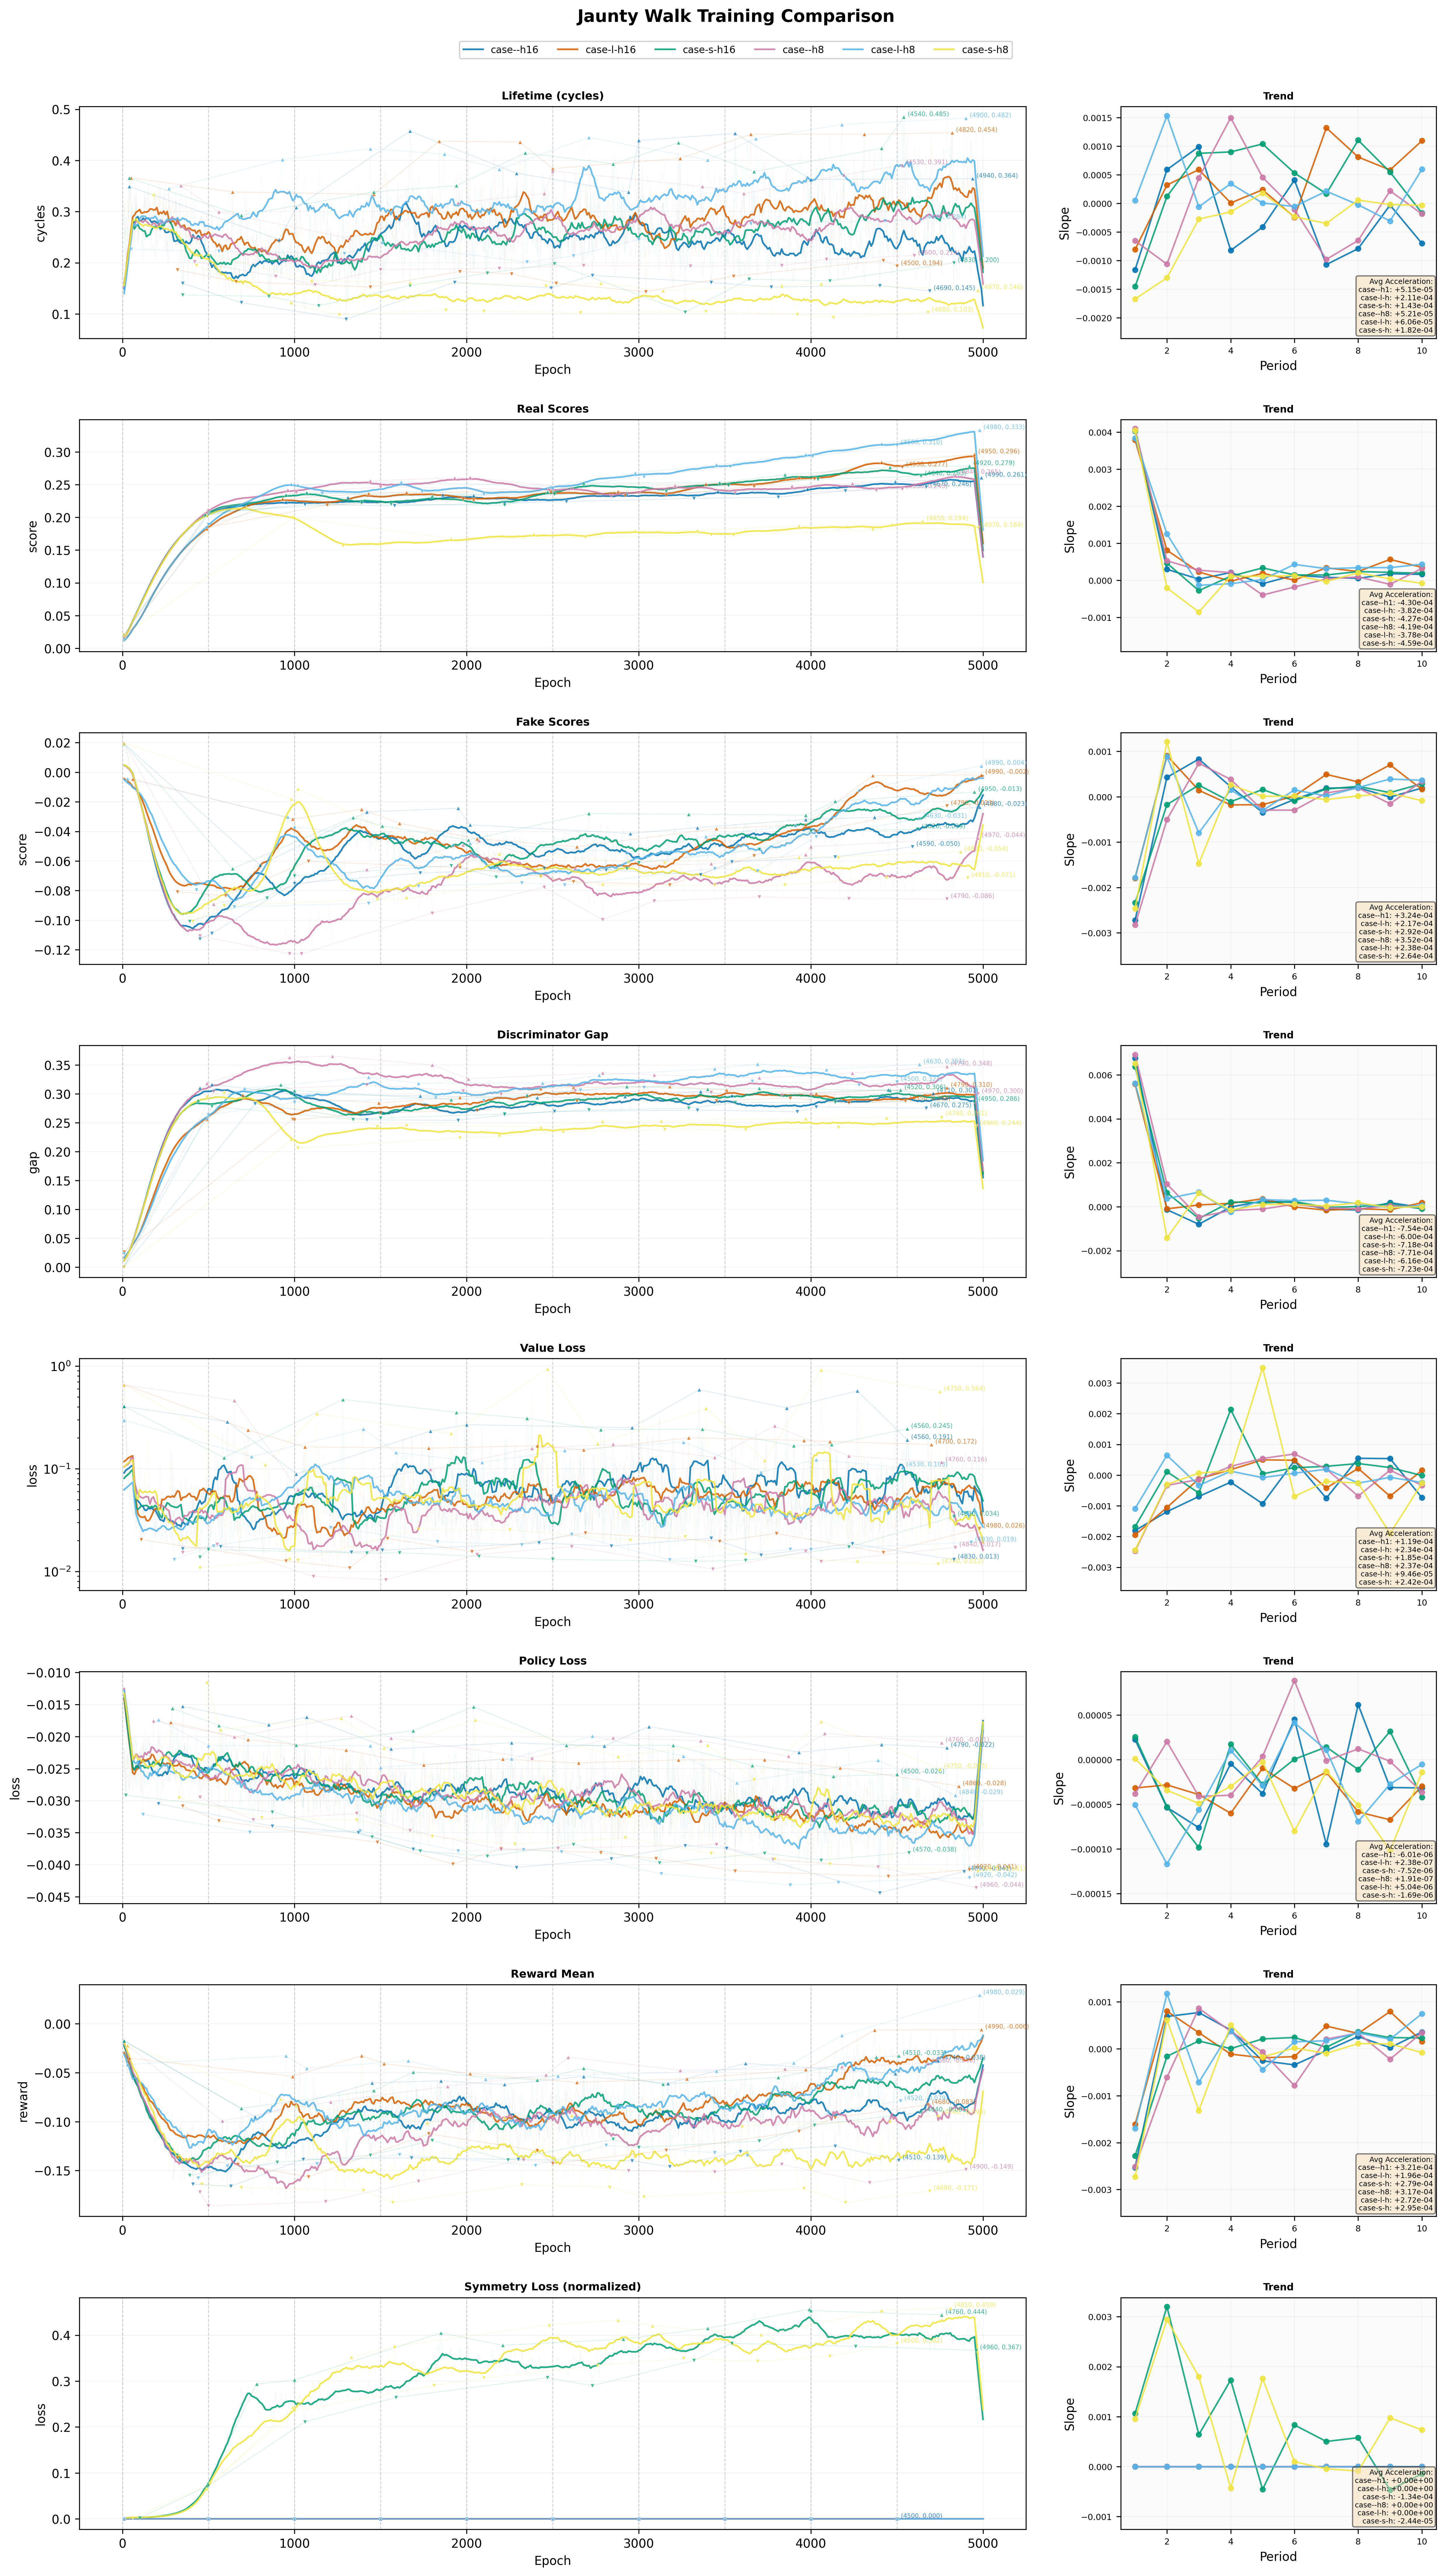
\includegraphics[height=.925\textheight, keepaspectratio]{outputs/case_studies/jaunty-h=8,16.png}
    \caption{Jaunty walk training comparison across experimental variants. The phase-conditioned variant (green) shows superior lifetime and reward characteristics for this asymmetric motion, while symmetry regularization (orange) degrades performance substantially.}
    \label{fig:jaunty_case}
\end{figure}

The mechanism operates as a \emph{temporal lookup key}: the policy queries which portion of the motion cycle it occupies and conditions its action distribution accordingly. This reduces variance in the advantage estimates for GAE and stabilizes early training. However, the conditioning assumes a known fixed cycle structure; it therefore generalizes poorly to aperiodic motions or multi-behavior transitions where $\phi_t$ becomes ill-defined.

\subsection{Case study II: bilateral symmetry regularisation}

The bilateral symmetry loss penalizes deviation from mirror symmetry across sagittal-plane joint pairs. For each left-right pair $(j^{\text{left}}, j^{\text{right}})$ with corresponding actions $(a_{j^{\text{left}}}, a_{j^{\text{right}}})$, the loss computes:
\[
    \mathcal{L}_{\text{sym}} = \frac{1}{N_{\text{pairs}}} \sum_{j \in \text{pairs}} \bigl\| (a_{j^{\text{left}}} - \bar{a}_j) - (a_{j^{\text{right}}} - \bar{a}_j) \bigr\|_2, \quad \bar{a}_j = \tfrac{1}{2}(a_{j^{\text{left}}} + a_{j^{\text{right}}}).
\]
The regularizer is applied with weight $\lambda_{\text{sym}} = 0.005$ during PPO updates, biasing the policy toward symmetric action distributions.

\textbf{Motion-dependent effects.} The regularizer's effectiveness depends on the inherent symmetry of the target motion:

\begin{enumerate}
    \item \textbf{Limp walk} (near-symmetric): At $H=8$, symmetry produced the best lifetime $0.71 \pm 0.08$ cycles; at $H=16$, remained competitive at $0.64 \pm 0.12$ cycles. The prior aligns well with the motion's near-symmetric ground contact pattern.
    
    \item \textbf{Jaunty walk} (asymmetric): The regularizer became strongly counterproductive:
    \begin{itemize}
        \item Lifetime dropped: $0.29 \pm 0.04 \rightarrow 0.13 \pm 0.01$ at $H=8$
        \item Normalized symmetry loss remained high: $0.4285 \pm 0.0158$
        \item The policy could not simultaneously minimize $\mathcal{L}_{\text{sym}}$ and match the asymmetric reference
    \end{itemize}
    
    \item \textbf{Joyful walk} (moderately asymmetric): Symmetry improved survival metrics but degraded imitation quality:
    \begin{itemize}
        \item Lifetime improved: $0.43 \pm 0.05 \rightarrow 0.71 \pm 0.08$ at $H=8$
        \item Fake discriminator score degraded: baseline $-0.03 \rightarrow -0.1043$ at $H=8$
        \item Same trade-off observed at $H=16$: lifetime $0.77 \pm 0.13$ but fake score $-0.0957$
    \end{itemize}
\end{enumerate}

\begin{figure}[htbp]
    \centering
    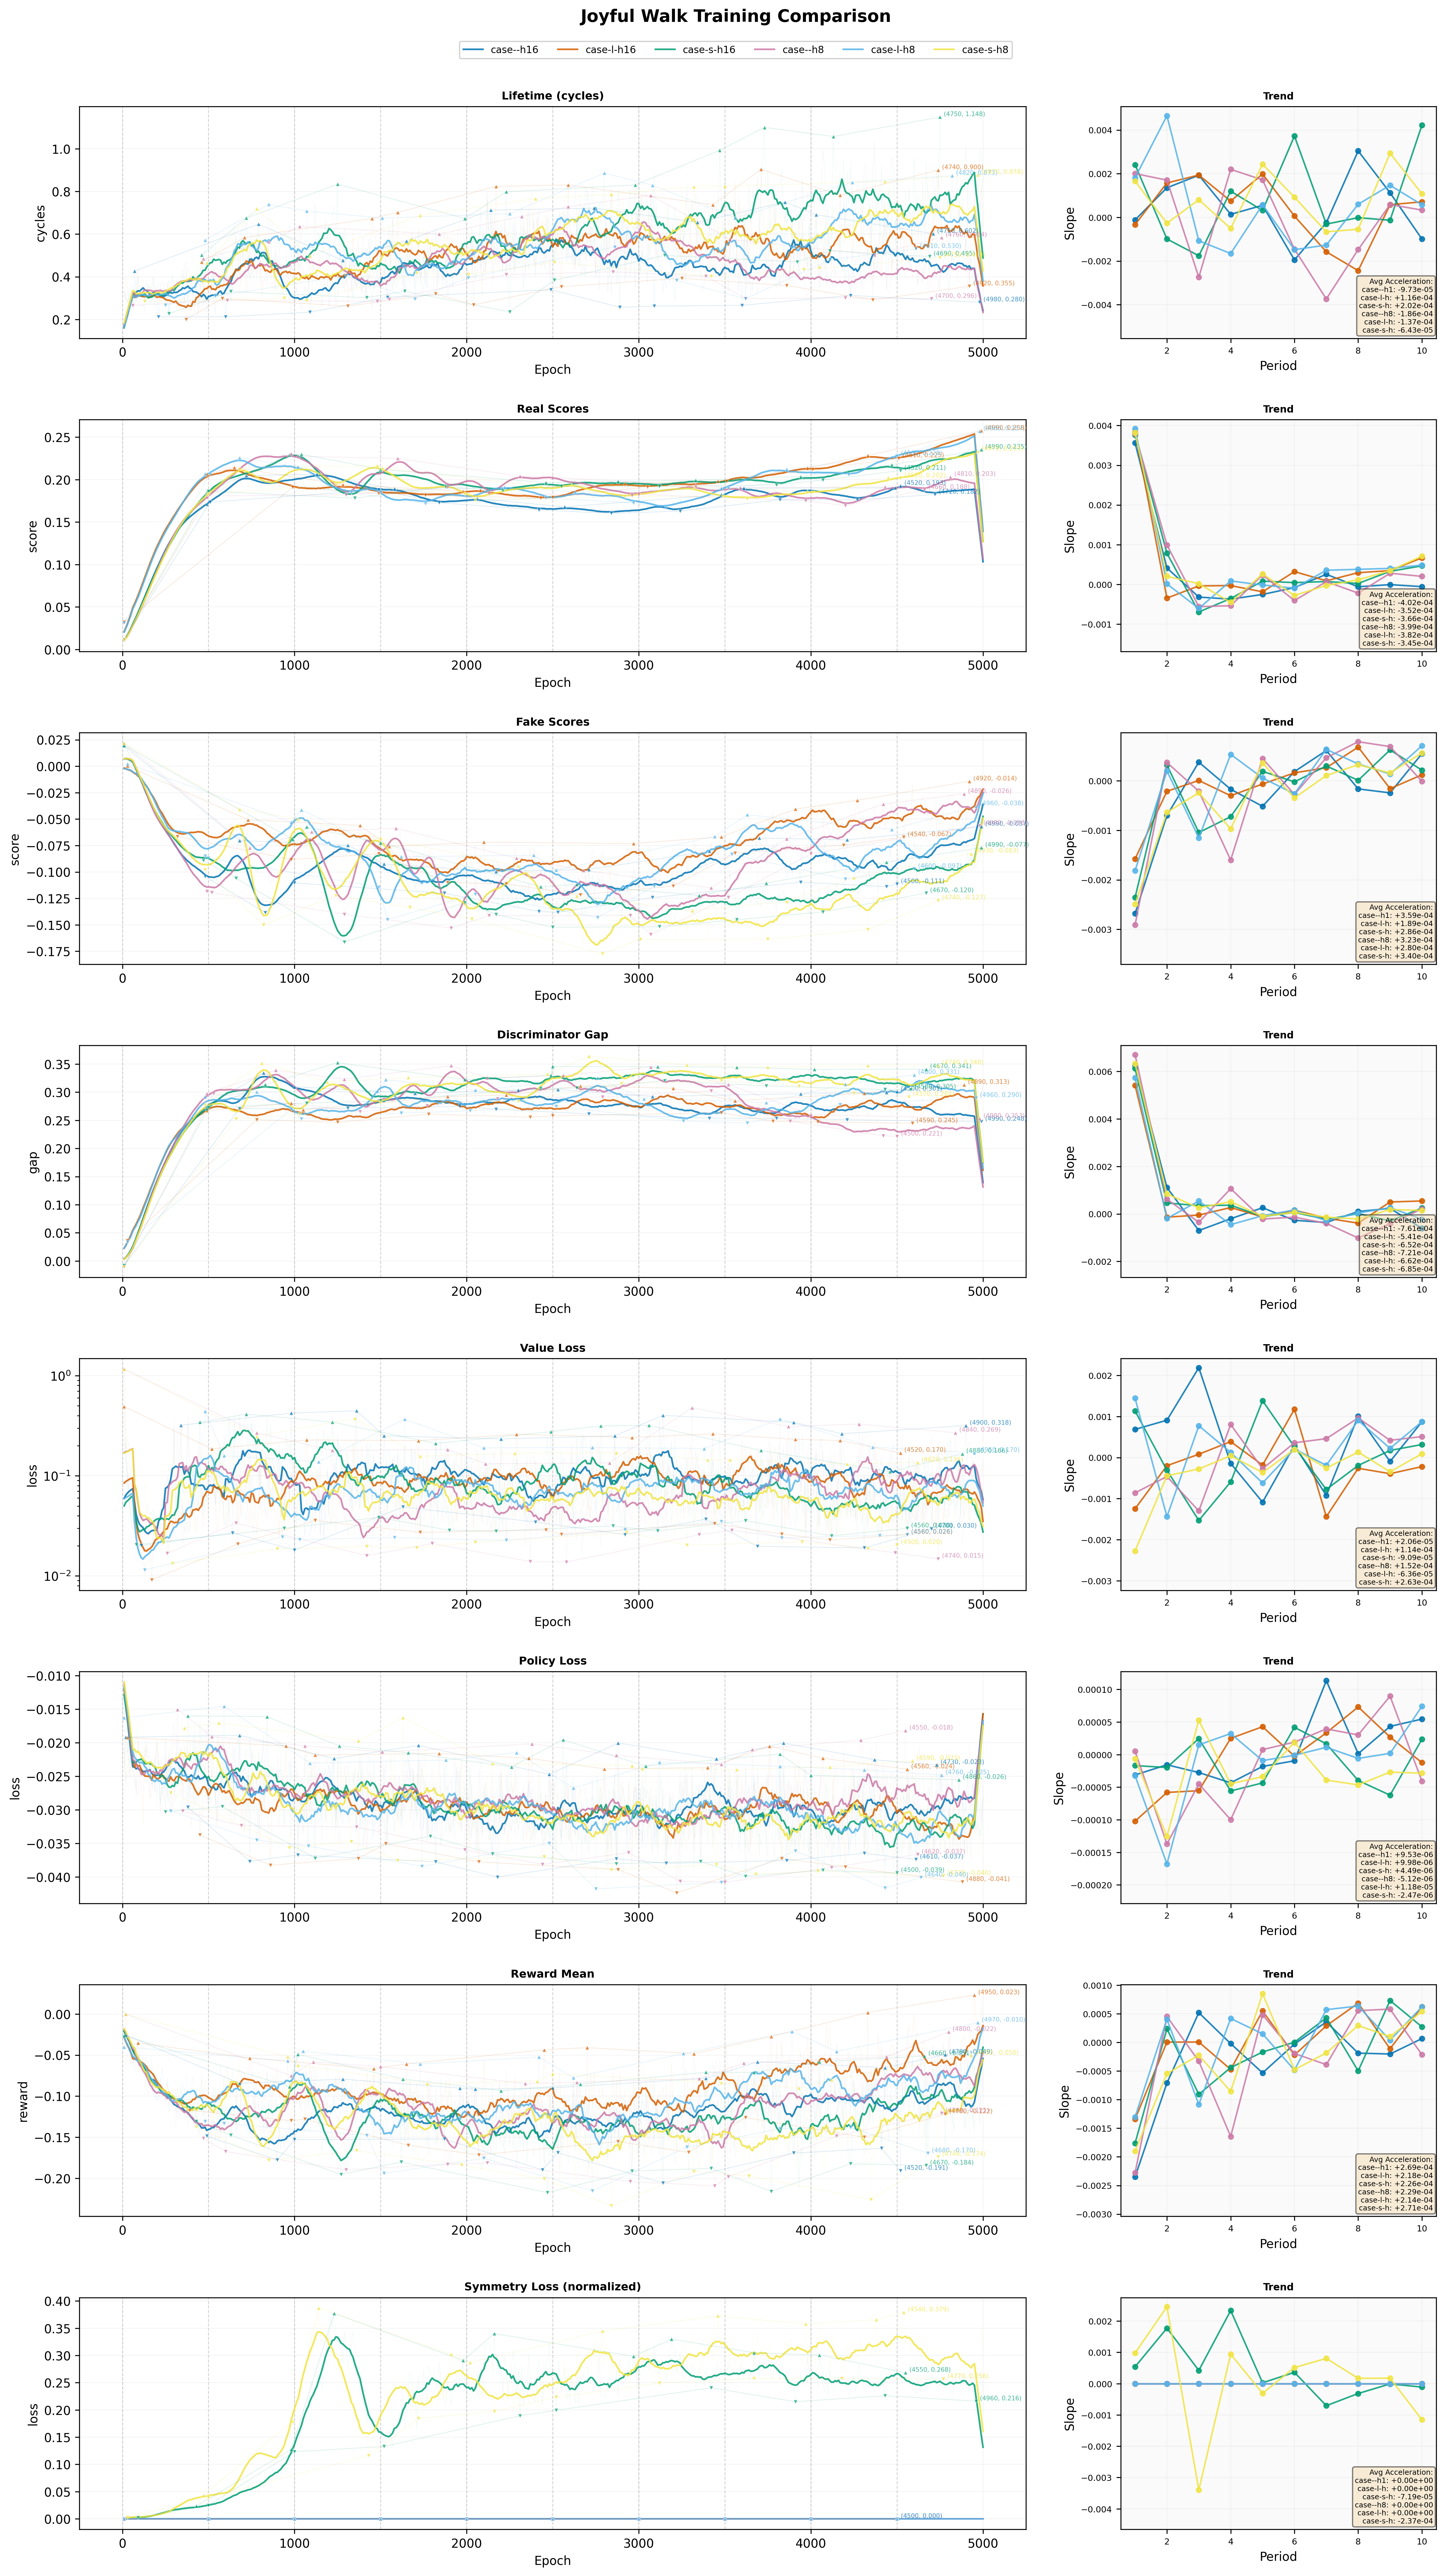
\includegraphics[height=.925\textheight, keepaspectratio]{outputs/case_studies/joyful-h=8,16.png}
    \caption{Joyful walk training comparison. The symmetry variant (orange) achieves high lifetime cycles but at the cost of discriminator quality (lower fake scores), indicating a survival-imitation trade-off.}
    \label{fig:joyful_case}
\end{figure}

\textbf{Interpretation.} The symmetry prior functions as an \emph{exploration bias} that constrains the action space to a lower-dimensional symmetric manifold. For near-symmetric gaits, this constraint excludes unstable asymmetric modes and accelerates convergence. For asymmetric motions, the constraint conflicts with the target distribution, producing either mode collapse (jaunty) or imitation-quality degradation (joyful). The appropriate application of this regularizer therefore requires \emph{a priori} knowledge of motion symmetry properties.

\paragraph{Pipeline use with generated motions.}
Beyond the controlled locomotion study, the pipeline was exercised on retargeted motion clips derived from the motion generator and stored under the `vimo` motion assets and checkpoints. These runs were used primarily as feasibility tests: they verified that the generated kinematic sequences could be converted into valid DeepMimic-style references and loaded by the MuJoCo controller without format mismatch. This experiment was important for the end-to-end objective of the project, because it established that the generated motions are not only visually plausible in kinematic space but also structurally compatible with the downstream control stack.

\subsection{Scope of the present study}
Only motion imitation and the two implemented ablations---phase-conditioned observations and bilateral symmetry regularisation---were evaluated systematically in the current work. Robustness experiments under perturbations, interactive policy switching, and fully goal-directed control were not implemented in the present pipeline and are therefore excluded from quantitative comparison here. Those components remain natural extensions once the imitation backbone is stabilized on a broader set of motions.

Default hyperparameters used throughout (overridable per config for task-specific parameters such as horizon, num\_envs, and grace\_steps):

\begin{table}[htbp]
\centering
\caption{Hyperparameters}
\begin{tabular}{ll}
\toprule
Parameter & Value \\
\midrule
policy network learning rate & $5 \times 10^{-6}$ \\
value network learning rate & $1 \times 10^{-4}$ \\
discriminator learning rate & $1 \times 10^{-5}$ \\
reward discount factor ($\gamma$) & 0.95 \\
GAE discount factor ($\lambda$) & 0.95 \\
surrogate clip range ($\epsilon$) & 0.2 \\
gradient penalty coefficient ($\lambda^{GP}$) & 10 \\
PPO replay buffer size & 4096 \\
PPO batch size & 256 \\
PPO optimization epochs & 5 \\
discriminator replay buffer size & 8192 \\
discriminator batch size & 512 \\
\bottomrule
\end{tabular}
\label{tab:hyperparams}
\end{table}

\begin{figure}[htbp]
    \centering
    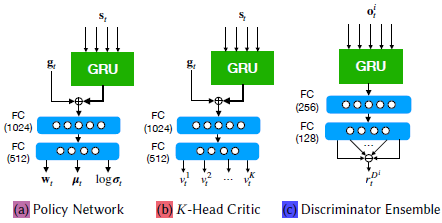
\includegraphics[width=.8\textwidth]{Pictures/exp_setup.png}
    \caption{Network architectures. $\oplus$ denotes the concatenation operator and $\ominus$ denotes the average operator.}
    \label{fig:network_arch}
\end{figure}

The adversarial controller follows the ICCGAN framework~\cite{iccgan2021} with a GRU-based policy network, K-head critic, and ensemble of body-part-specific discriminators. The policy maps state to action distribution via GRU + fully-connected layers; the critic estimates values per discriminator head; the discriminator ensemble distinguishes reference from generated trajectories on joint subsets. Average operator ($\ominus$) aggregates features while concatenation ($\oplus$) fuses state and goal inputs. This architecture eliminates manual reward engineering by letting the policy learn to fool the discriminators directly.